\section{History of Scientific Auroral Observations}\label{sec:historyaurora}

Targeted observational efforts dedicated to aurora extended throughout the eighteenth and nineteenth centuries, noting several distinct colors and morphologies of various auroral forms \citep{wilcke1778,schwickert1833}.
Quantitative observations of auroral spectra required moving beyond Newton's seventeenth century prism experiments to get sufficient sensitivity and selectivity.
Eighteenth century prism and thermometer experiments \citep{herschel1800} were adequate to reveal the large infrared component of the solar spectrum, but were far too insensitive for quantitatively measuring spectra of non-solar features in the sky.
Rapid iteration by several researchers from about 1800--1850 opened the path for \AA ngstrom's founding role in scientific spectroscopy of quantitative solar observations \citep{reifacherman2014}.
Following the \citet{angstrom1869} reported measurement of \unit[557.7]{nm}, spectral measurements by \citet{fritz1881} recorded several emission lines, but with substantial wavelength error versus the much higher fidelity methods employed in 1899-1900 \citep{sykora1901,chernouss2005}.
The correct identification of atomic oxygen O responsible for the yellow-green \unit[557.7]{nm} line typically brightest at auroral latitudes (60..70$^\circ$ N) did not occur until 1923 \citep{chernouss2008}.

Instrumentation developed and distributed by \citet{rayleigh1924} established the global ubiquity of airglow and its distinction from aurora via carefully calibrated three-broadband filter arrangements.
Quantitative analysis of auroral intensity versus wavelength was accelerated in the latter half of the twentieth century \citep{seaton1954} as equipment improved and the theory rapidly evolved via increased observational efforts.
Theoretical predictions by \citet{garstang1951} for long-lived metastable [OI]32 \unit[557.7]{nm} lifetime $\sim \unit[0.7]{s}$ were observationally confirmed by \citet{omholt1955} using the apparatus of Figure~\ref{fig:omholtpmt}.
\begin{figure}\centering
    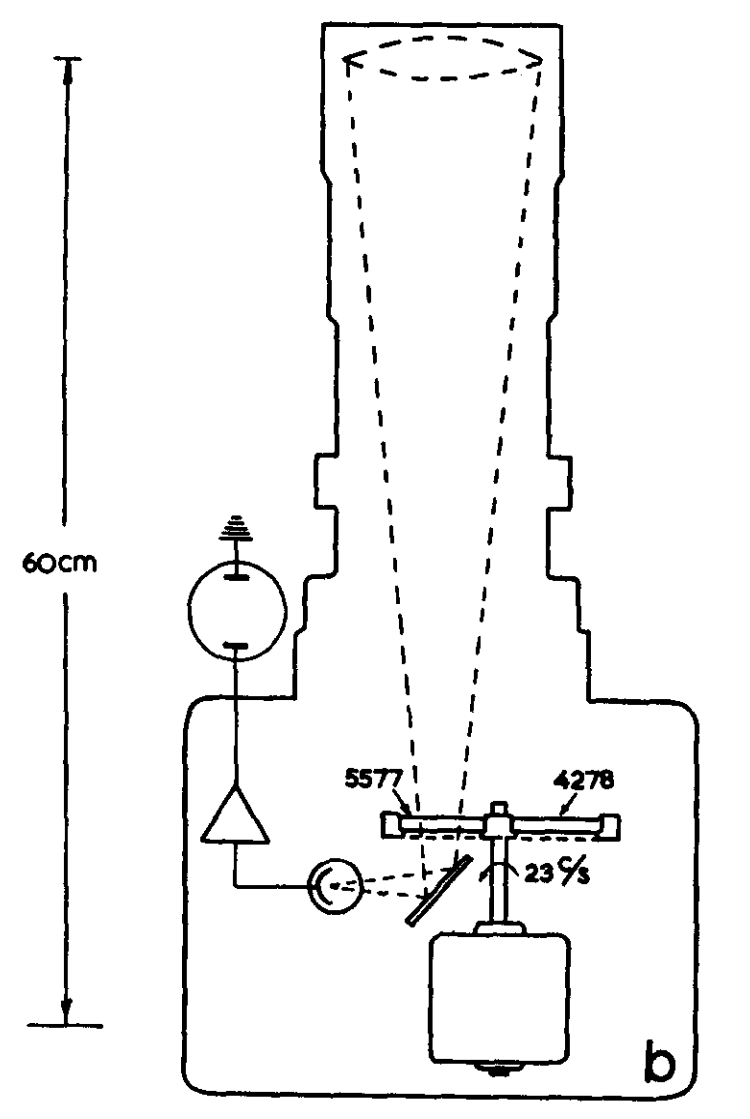
\includegraphics[width=0.6\linewidth]{gfx/omholtpmt}
    \caption{\citet{omholt1955} apparatus for \unit[23]{Hz} measurements in Tromsø during autumn 1954 of prompt \unit[427.8]{nm} emissions compared with forbidden long-lifetime \unit[557.7]{nm} emissions using a PMT to CRT and recorded on film strip.}\label{fig:omholtpmt}
\end{figure}
Stable auroral red (SAR) \unit[630.0]{nm} aurora with an absence of the \unit[557.7]{nm} emission common to polar aurora and airglow was discovered in 1956 with more sensitive imaging techniques \citep{baumgardner2007}.
Theoretical \unit[630.0]{nm} lifetime was likewise measured \citep{stoffregen1960} to be $\sim \unit[110]{s}$ via auroral spectrograph, since this lifetime would be exceedingly difficult to measure in an anthropogenic laboratory.
Extensive spectral work in the 1960s \citep{broadfoot1968} revealed high resolution relative intensities and corresponding chemistry of emissions that Rayleigh and associates broke into three coarse visible bands.
As aeronomical efforts expanded, the spectrum \citep{rees1974} and morphology of aurora were quantitatively and repeatably measured throughout the latter twentieth century \citep{nagy2015}.
Continued advances in spectroscopy led to fine quantification of auroral emission bands.
Laboratory verification of the lifetimes and other characteristics of kinetic reactions driving the optical emissions was enabled by instruments \citep{barrett1976} like that shown in Figure~\ref{fig:BellJar}.
\begin{figure}\centering
    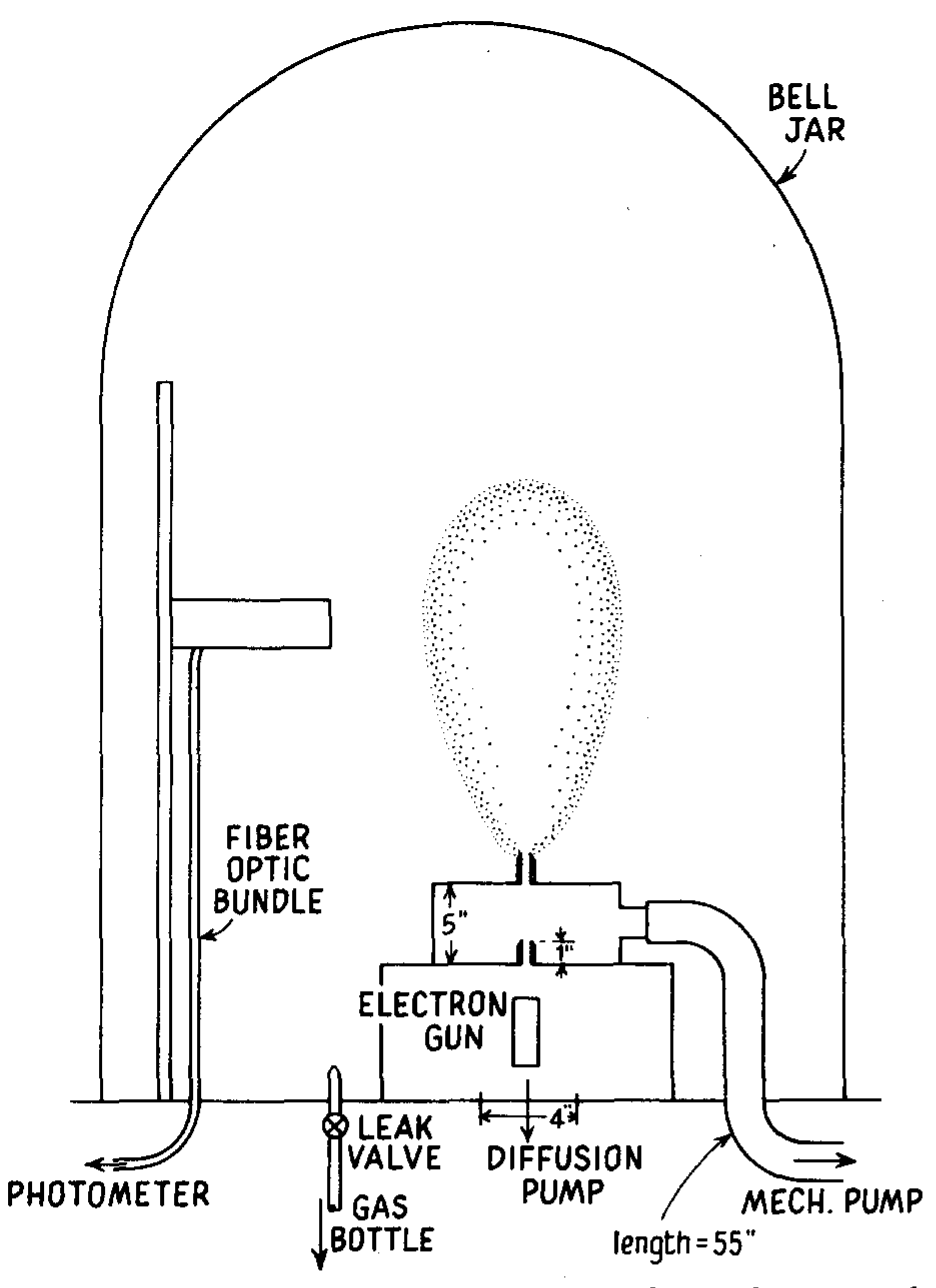
\includegraphics[width=0.5\textwidth]{gfx/BarrettHaysBellJar}
    \caption{Electron penetration depth measurement mechanism used by \citet{barrett1976}}\label{fig:BellJar}
\end{figure}

\subsection{Twenty-first Century Auroral Observation}

As the twenty-first century dawned, auroral tomography first focused on reconstructing VER \citep{bjorn1998} $\sim \unit[1]{Hz}$ in concert with wide-angle camera networks \citep{donovan2006}.
As personal computing power underwent explosive growth, desktop 1-D ionospheric particle precipitation dynamics models \citep{blelly1996a} began to enable tying together ISR and optical observations across a wide range of wavelengths \citep{zettdis,dahlgren2013}.
Automated networked observatories have become the new way forward in geoscience and particularly in geospace.
This dissertation describes instruments developed to enable the cutting edge of ionospheric plasma science.

